\chapter{ACTUAL WORK} % Main chapter title
\label{ChapterActualWork} % For referencing the chapter elsewhere, use \ref{Chapter1} 


Upon completion of identifying \& formulating the research problem, and carrying out the necessary literature survey and review, the actual work on the project is taken-up. This chapter is dedicated to the actual work done by students. Hence, the chapter name and sub-chapter names are not fixed. It is left to the discretion of the students with appropriate guidance from their respective supervisors. However, one or more of the following aspects (as applicable) shall be covered in this chapter:
\begin{itemize}
	\item Methodology of the study or actual work (different from research methodology)
	\item Experimental and/or analytical work completed in the project
	\item Modeling, Analysis and Design
	\item Prototype and testing
\end{itemize}

In this project, I help design and build a web-site that is visually pleasing to all the age groups and has a great user experience. This website is designed to emulate how an offline exhibit would be like. A lot of work went into the design and the user experience of the website, and then more during web development. Various applications, and web-development technologies were utilized to create this online exhibit. 

% \Section{Software Requirements}\index{Software Requirements}

Software Requirements
\\
\textbf{Adobe XD}
Adobe XD is a vector-based digital design tool for websites and apps. It is used to  create and collaborate on everything from prototypes to mockups to full designs. It is developed by Adobe and is available for Windows and macOS. It supports website, mobile, apps,etc to create wireframes and click-through prototypes.


\textbf{Framer X}

\textbf{React Js}

\textbf{Tailwind CSS}

\textbf{ Frame Motion }

\textbf{Google Sheet API}

\textbf{React Slick - used in creating the custom slider}






\section{Methodology for the Study}\index{Methodology}

The purpose of creating a website for the online exhibition is to provide a medium for students, researchers, and scholars to gather and get to know about the research of various other scientists/researchers from various other fields. The first step to do that is to make the website have a very good user experience and that can be used by all age groups, and also make is simple yet elegant in the views of these users. This is done by a lot reserach of the way the various interactionms can be shown and also the best way to show details of a particular exhibit. 

\section{Experimental and or Analytical Work Completed in the Project}

\textbf{Using React Slick to create a custom slider}
\\
React slick is a react component that can be used to create custom carousel's based on various parameters and CSS tweaking. React-Slick by itself is a component made up of javascript and css which has a basic slider functionality that we have used in this project to create the main page by customizing it a lot. The reason to choose this project over any other was because of the simplicity and the accessibility to its parent code that is provided to us when we install it. 

\textbf{Google Sheets API}
\\
Google sheets API provides us a way to Read, write, and format data in Sheets using the their API. This API has a lot of settings with which we can create beautiful and functional sheets within the code itself. Each spreadsheet has an id associated to it(you can also have a look at this id in the url when you open a google spreadsheet).
The main reason we choose this API was to read the cells of the spreadsheet, so that data from here can be populated in the exhibition website.  

\section{Modeling, Analysis \& Design}

\section{Prototype \& testing}

\section*{Sample LaTeX Typesetting}


\paragraph*{Figure} Vector Graphics EPS Format [Figure \ref{fig:fcmc1}]
\begin{figure}[H]
	\begin{center}
		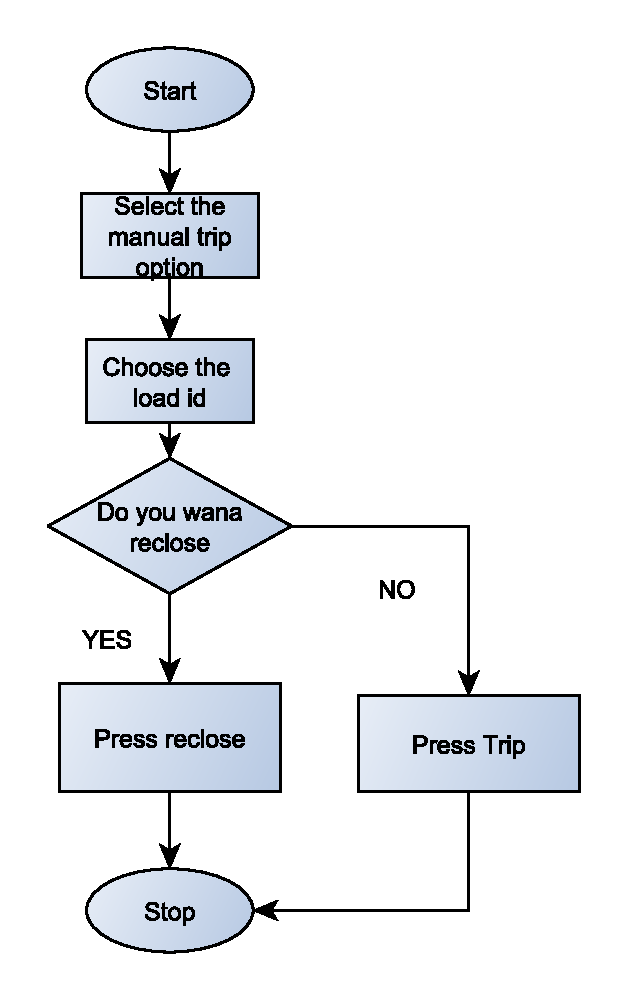
\includegraphics[scale=0.5]{Figures/manualtrip.eps}
		\caption{Flowchart of Manual Controller}
		\label{fig:fcmc1}
	\end{center}
\end{figure}


\paragraph*{Figure} JPEG/JPG Format [Figure \ref{fig:rb}]
\begin{figure}[h]
	\begin{center}
		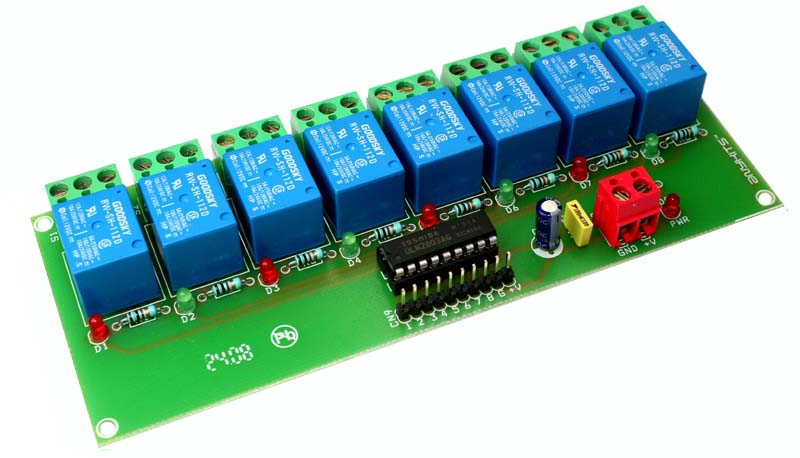
\includegraphics[scale=0.3]{Figures/relay.jpg}
		\caption{Relay Board}
		\label{fig:rb}
	\end{center}
\end{figure}

\paragraph*{Table} Refer [Table \ref{tab:sm}]
\begin{table}[h]
	\centering
	\caption{Student Marks}
	\begin{tabular}{rr}
		\toprule
		Name  & Marks \\
		\midrule
		Ajay  & 10 \\
		Vinay & 20 \\
		\bottomrule
	\end{tabular}%
	\label{tab:sm}%
\end{table}%


\paragraph*{Cross References: Citation, Index, Reference, Equation reference}
This is the methodology for the entire project work which includes even the process of deciding on the project title, objectives
\index{Ojectives}, etc. This is mandatory for MTech and optional for BTech)\cite{abcdef}. The data is shown in Table \ref{tab:sm}. The equation shown in Equation \eqref{Eq:eq123}

\paragraph*{Inline Equation}
This is my equation.
$	f = ma \pm \alpha \Delta \left[ {\begin{array}{*{20}{c}}
	1 & \chi   \\
	{ - 1} & 0  \\
	\end{array}} \right] $
,which is appearing in between some text.

\paragraph*{Equation without Numbering} 
\begin{equation*}
	x = \frac{{ - b \pm \sqrt {{b^2} - 4ac} }}{{2a}}\
\end{equation*}

\paragraph*{Equation with Numbering} 
\begin{equation} \label{Eq:eq123}
\dot X = \left[ {\begin{array}{*{20}{c}}
	1 & p  \\
	2 & \alpha   \\
	\end{array}} \right]\left[ {\begin{array}{*{20}{c}}
	{{x_1}}  \\
	{{x_2}}  \\
	\end{array}} \right] + Bu\
\end{equation}



\paragraph*{Algorithm Format} 
\begin{algorithm}
	\caption{Addition of two 8 bit numbers}\label{alg:add8bit}
	\begin{algorithmic}[1]	
		\\ Start
		\\ Input a and b
		\\ c=a+b
		\\ Output c
		\\ stop
	\end{algorithmic}
\end{algorithm}


\paragraph*{Enumeration Format}
The following are the different flavor of Tex systems
\begin{enumerate}
	\item TeXLive TeX System
		\begin{enumerate}
			\item TeXLive for Windows
			\begin{enumerate}
				\item TeXLive
				\item ProTex
			\end{enumerate}
			\item MacTeX for Mac
		\end{enumerate}
	\item MikTeX TeX System
\end{enumerate}

\paragraph*{Bullets Format}
The following are the advantages of LaTeX,
\begin{itemize}
	\item {\LaTeX} is highly portable and free.
	\begin{itemize}
		\item Contribute to TUG
		\item Promote Free Softwares
	\end{itemize}
	\item Operating-system independent.
	\item Complex scientific documents can be created
	automatically.
	\item High quality math typesetting.
\end{itemize}

\paragraph*{Program Inclusion} Program file present in other directory can be embedded into the report.
\lstinputlisting{Files/code.asm}

\paragraph*{Verbatim Text} Include text as it is.
\\
The additional database schema is shown below which is used to store all the configuration and transaction data.
\begin{verbatim}
CREATE TABLE `controller_config` (
`load_id` int(11) NOT NULL,
`ct_constant` double DEFAULT NULL,
`pt_constant` double DEFAULT NULL,
`samples` int(11) DEFAULT NULL,
`delay` double DEFAULT NULL,
PRIMARY KEY (`load_id`)
) ENGINE=InnoDB DEFAULT CHARSET=utf8;
SELECT * FROM loadcontroller.load_details;
\end{verbatim} 


